\section{Fase di implementazione}
\label{sec:fase_di_implementazione}
\subsection{Linguaggi}
\subsubsection{HTML}
Tutte le pagine del sito sono state realizzate utilizzando come linguaggio di markup XHTML piuttosto che HTML5, per garantire un certo grado di qualità del codice e alta compatibilità con i browser più obsoleti. In particolare le differenze più importanti che ci hanno portato a preferire XHTML ad HTML5 sono:
\begin{itemize}
	\item I tag \htmlcode{<html>}, \htmlcode{<head>}, \htmlcode{<title>} e \htmlcode{<body>} sono obbligatori;
	\item Gli elementi devono essere nidificati correttamente;
	\item Gli elementi devono essere sempre chiusi;
	\item Gli elementi devono essere sempre in minuscolo;
	\item I nomi degli attributi devono essere sempre in minuscolo;
\end{itemize}
Per le form di registrazione e accesso, abbiamo scelto di utilizzare come input per le e-mail il tipo \htmlcode{text}, che grazie ad opportuni controlli specificati nelle sezioni \S\ref{subs:php} e \S\ref{subs:javascript}, si comporta quasi similmente al tipo \htmlcode{email} di HTML5. Allo stesso modo, anche gli input che riguardano il tempo di una ricetta, la difficoltà di una ricetta e la barra di ricerca, sono tutti di tipo \htmlcode{text} al posto dei tipi \htmlcode{number}, \htmlcode{range} e \htmlcode{search}.

\subsubsection{CSS}
Per la definizione della presentazione del sito è stato utilizzato CSS3 puro. Per mantenere la separazione tra contenuto e presentazione, non sono stati utilizzati tag di stile in XHTML ma sono stati utilizzati fogli di stile esterni. \\
Le regole utilizzate sono state valutate in base alla compatibilità con i diversi browser, eventuali regole applicate non compatibili con Internet Explorer (in particolare \textit{object-fit}) non compromettono le funzionalità del sito o l'esperienza dell'utente. \\
Per mantenere un design fluido e scalabile sono state preferite le unità di misura relative a quelle assolute ed è stato utilizzato il Flexbox Layout per garantire flessibilità al design.

\subsubsection{SQL}
Il database mantiene le informazioni strutturali sulle ricette, comprese metainformazioni come l'autore della pagina, e le informazioni di accesso sugli utenti.
Inoltre, mantiene i voti e i commenti degli utenti.
Lo schema relazionale del database è:

\begin{figure}[h!]
	\centering
	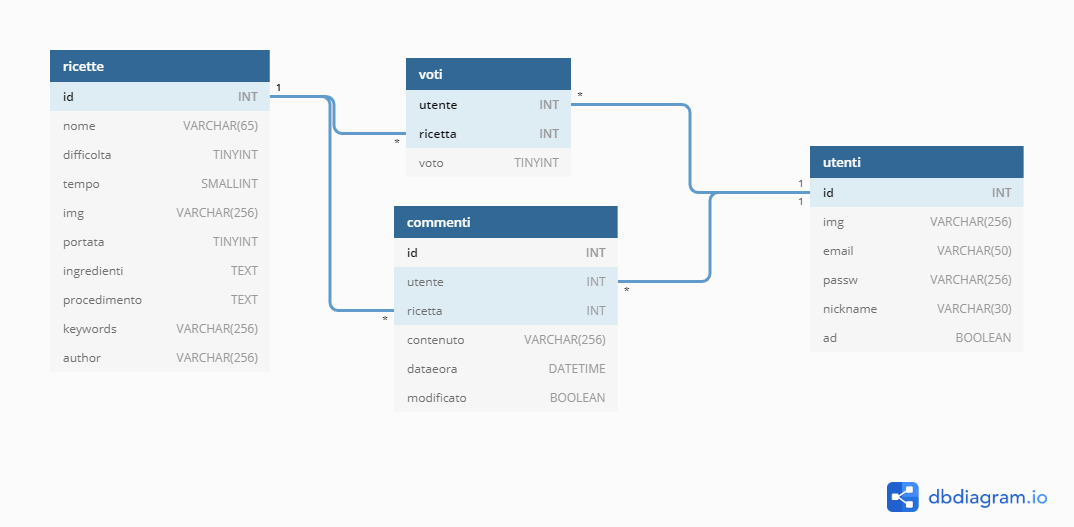
\includegraphics{img/progettazione/schema-db}
\end{figure}

Le chiavi primarie delle tabelle sono degli identificatori numerici autoincrementali, eccetto per \sqlcode{voti}, per la quale la chiave primaria è data dall'utente che ha dato il voto e la ricetta che è stata votata, entrambi chiavi esterne.
Essendo plausibili più commenti dello stesso utente alla stessa ricetta, non abbiamo potuto utilizzare la stessa soluzione per la tabella \sqlcode{commenti}, per la quale sarebbe stato necessario includere anche l'orario, possibilità preclusa da \textit{MariaDB}.

Oltre alle chiavi primarie, abbiamo imposto un vincolo di unicità sul nome delle ricette e su nome utente ed email degli utenti, per evitare inutili confusioni in caso di ripetizioni.
Per prevenire riferimenti a contenuti rimossi, all'eliminazione di una ricetta o un utente vengono eliminati anche i rispettivi commenti e voti.

\subsubsection{PHP}\label{subs:php}
\paragraph{Costruzione delle pagine}
Tutte le pagine del sito sono costruite dinamicamente.
Abbiamo definito la struttura essenziale comune a tutte le pagine attraverso un template, utilizzando degli elementi vuoti invalidi (i cui tag sono riconoscibili immediatamente grazie al suffisso \htmlcode{Placeholder}) per rappresentare porzioni dell'albero XML diverse fra le pagine.
Queste porzioni dinamiche sono definite in appositi file separati; le funzioni \phpcode{file_get_contents($filename)} e \phpcode{str_replace($search,$replace,$subject)} permettono di inserire il contenuto di tali file in sostituzione ai tag invalidi, ottenendo un documento completo e valido.
In alcuni casi, per semplificare la costruzione delle pagine, anche i file parziali contengono tag invalidi, i quali vengono sostituiti applicando ricorsivamente la stessa procedura.
Abbiamo scelto di utilizzare l'estensione \textit{.php} per tutti i file contenenti tag invalidi, per evidenziare la loro non completezza e non validità.
Fra i tag invalidi, due sono di particolare rilevanza:
\begin{itemize}
	\item \htmlcode{<rootFolder />} viene utilizzato per indicare un path relativo alla pagina corrente della radice del sito.
	\item \htmlcode{<backToTopPlaceholder />} indica la posizione di un link \textit{Torna Su}.
\end{itemize}
Questi due tag possono essere utilizzati in tutti i file, e vengono sostituiti con il rispettivo codice valido solo al termine di tutte le altre sostituzioni.

Per una comoda gestione del template principale, abbiamo definito una classe \phpcode{DBConnection}.
Ogni script che deve ritornare una pagina al client istanzia questa classe, ed invocando i suoi metodi la costruisce.
Sono disponibili i metodi:
\begin{itemize}
	\item \phpcode{__construct($root,$standard)} per costruire un'istanza della classe. \phpcode{$root} deve essere il path relativo alla directory corrente della directory radice del sito, cioè quella contenente il file \texttt{index.php}. \phpcode{$standard} deve essere la stringa \phpcode{"xhtml"}. In origine era prevista la possibilità di scelta fra gli standard XHTML e HTML5 in base alla pagina attraverso questo parametro; dopo avere scelto di utilizzare solo XHTML, abbiamo comunque mantenuto questo parametro a fini di  manutenibilità ed estensibilità.
	\item \phpcode{setTitle($title)} per inserire il titolo della pagina, sia nel tag \htmlcode{title} sia nel tag \htmlcode{meta} con \htmlcode{name="title"}.
	\item \phpcode{setDescription($description)} per inserire la descrizione della pagina nel tag \htmlcode{meta} con \htmlcode{name="description"}.
	\item \phpcode{setAuthor($author)} per inserire il nome dell'autore della pagina nel tag \htmlcode{meta} con \htmlcode{name="author"}.
	\item \phpcode{setOtherMeta($tags)} per inserire altri tag \htmlcode{meta}.
	\item \phpcode{setLogin($loginSnippet)} per inserire i link alle pagine di login e signup se l'utente non è autenticato, oppure un messaggio di benvenuto, il link alla pagina utente ed il link per il logout se è autenticato.
	\item \phpcode{setNav($navSnippet)} per inserire il menu, i cui link possono venire rimossi per evitare riferimenti circolari.
	\item \phpcode{setBreadcrumb($breadcrumbSnippet)} per inserire il breadcrumb specifico per ogni pagina.
	\item \phpcode{setContent($contentSnippet)} per inserire il contenuto della pagina.
	\item \phpcode{setBackToTop($backToTopSnippet)} per inserire i link \textit{Torna Su}.
	\item \phpcode{setAnnulla($annullaSnippet)} per inserire i pulsanti \textit{Annulla}.
	\item \phpcode{setFooter($footerSnippet)} per inserire il footer del sito
	\item \phpcode{send()} per completare l'elaborazione ed inviare la pagina completa al client.
	\item \phpcode{save($file)} per completare l'elaborazione e salvare la pagina completa su file.
\end{itemize}

\paragraph{Autenticazione}

L'autenticazione è gestita attraverso il sistema delle sessioni, fornito nativamente da PHP\@.
Un utente è rappresentato da un'istanza della classe \phpcode{User}, che acquisisce dal database i dati dell'utente al momento del login e li espone attraverso appositi metodi getter.
Quando questa classe viene istanziata, l'oggetto risultante viene salvato nella entry \phpcode{user} della variabile superglobale \phpcode{$_SESSION}, per permetterne l'accesso da qualunque script.
Quando l'utente esegue il logout, la sessione viene resettata attraverso le funzioni \phpcode{session_unset()} e \phpcode{session_destroy()}, che eliminano tutte le informazioni di sessione salvate.

\paragraph{Pagine di errore}

Per segnalare all'utente errori nelle richieste al server, causati ad esempio dall'inserimento di un URL incorretto, abbiamo implementato delle pagine di errore corrispondenti ai codici HTTP rilevanti per il sito, in particolare per gli errori lato client.
Ogni pagina di errore è implementata in un file nella radice del sito nominato \texttt{XXX.php}, dove \texttt{XXX} è il rispettivo codice HTTP\@.

\begin{itemize}
	\item Errore \textit{400 BAD REQUEST}: ritornato nel caso l'URL della richiesta non rispetti vincoli di coerenza, ad esempio l'esecuzione di una ricerca priva del termine della ricerca nella query.
	\item Errore \textit{401 UNAUTHORIZED}: ritornato nel caso in cui sia necessaria un'autenticazione non fornita, ad esempio cercando di inserire un commento prima di aver eseguito il login.
	\item Errore \textit{403 FORBIDDEN}: ritornato nel caso in cui l'utente sia autenticato, ma non abbia i permessi necessari ad eseguire l'operazione richiesta, ad esempio cercando di inserire una nuova ricetta senza essere un amministratore.
	\item Errore \textit{404 NOT FOUND}: ritornato nel caso in cui la richiesta abbia una sintassi non riconosciuta, ad esempio se l'URL individua un file non esistente.
\end{itemize}

\paragraph{Funzionalità di ricerca}

Da tutte le pagine del sito è possibile accedere alla barra di ricerca, che esegue una ricerca \textit{case insensitive} del termine ricercato in tutti i titoli delle ricette.

\paragraph{Query al database}

Per migliorare la modularità del codice, abbiamo implementato delle funzioni atte ad eseguire le query al database più importanti del sito, le quali costruiscono anche il rispettivo codice HTML.
Le funzioni, raccolte nel file \texttt{query-portata.php}, sono
\begin{itemize}
	\item \phpcode{contentPortata($portata, $min, $num)}, che ritorna una lista di ricette della portata indicata da \phpcode{$portata}. Le ricette sono ordinate per età crescente, e vengono ritornate solo \phpcode{$num} ricette a partire dalla \phpcode{$min}-esima, per permettere la paginazione.
	\item \phpcode{contentRicerca($termine, $min, $num)}, che ritorna, in modo completamente analogo a \phpcode{contentPortata}, una lista di ricette il cui titolo contiene il termine di ricerca.
	\item \phpcode{piattoMigliore($portata)}, che ritorna la ricetta della portata indicata da \phpcode{$portata} con il voto (medio) più alto.
\end{itemize}

\paragraph{Moduli di inserimento e modifica}

Per l'elaborazione dei dati inseriti dall'utente sono presenti degli script, contenuti in file riconoscibili per il prefisso \texttt{handle} nel nome del file.
Per quanto riguarda l'inserimento e la modifica di ricette, prerogative degli utenti con permessi di amministratore, è disponibile una forma semplice di markup per indicare parole in lingue diverse dall'italiano.
Le espressioni markup vengono salvate nel database, e vengono convertite a codice HTML solo al momento della costruzione della pagina da ritornare al client.

\paragraph{Validazione lato server}\label{par:validazione_lato_server}
Le funzioni di validazione degli input lato server sono contenute all'interno del file \texttt{validation.php}. I controlli implementati si comportano allo stesso modo di quelli descritti nella sezione \S\ref{subs:javascript} aggiungendo loro il controllo anche dei dati presenti nel database, nello specifico:
\begin{itemize}
	\item \phpcode{checkNickname($stringNickname)} che oltre a controllare se l'input inserito dall'utente contiene non più di 20 caratteri alfanumerici, controlla anche che il nome non sia già presente nel database.
	\item \phpcode{checkEmail($stringEmail)} che valida la mail grazie al filtro offerto da PHP e inoltre controlla che la mail non sia già presente nel database.
	\item \phpcode{comparePassword($stringPassword, $stringPasswordConfirm)} che verifica, se entrambi i campi non sono vuoti, che le due password siano uguali tra loro.
	\item \phpcode{checkLogin($stringPassword, $stringNickname)} controlla che sia il nickname che la password inseriti dall'utente non siano stringhe vuote, che il nickname inserito sia presente nel database e che ad esso corrisponda la passowrd immessa dall'utente.
	\item \phpcode{checkNomeRicetta($stringNomeRicetta, $dbCondition)} che varifica se la stringa rispetta la lunghezza di massimo 55 caratteri alfanumerici e, se la variabile \phpcode{dbCondition} è true, anche che il nome non sia già presente nel database. Quest'ultimo controllo viene fatto solo nel caso si sia aggiungendo una nuova ricetta, mentre non viene fatto se si vuole modificare una ricetta senza cambiarne il nome.
	\item \phpcode{checkDifficolta($stringDifficolta)} controlla che la stringa che rappresenta la difficoltà sia un numero tra 1 e 5.
	\item \phpcode{checkTempo($stringTempo)} verifica che il tempo non sia vuoto e che sia un intero positivo, escluso lo zero.
	\item \phpcode{checkKeywords($stringKeywords)} controlla che la stringa inserita dall'utente non sia vuota e che contenga almeno un carattere alfanumerico.
	\item \phpcode{checkImage($stringImage)} verifica che il file caricato sia effettivamente un'immagine controllando la sua estensione, e che la sua dimensione non superi 150KB.
	\item \phpcode{checkCommento($testo)} che controlla grazie all'espressione regolare, che il testo del commento non sia vuoto. Non è stato utilizzato la funzione \phpcode{empty()} perchè la stringa \phpcode{"0"} veniva considerata come vuota, mentre contiene un carattere.
\end{itemize}
Inoltre è stata implementata una funzione ausiliaria \phpcode{test_input($data)} che rimuove sia gli spazi che gli slash di escape, e trasforma in html i caratteri speciali, per esempio \phpcode{à} diventa \phpcode{&agrave;}.
Ogniqualvolta un utente digiti erroraneamente dei dati che non rispettano almeno una validazione, viene informato mediante l'opportuna stampa degli errori e i dati inseriti vengono mantenuti negli input delle form grazie al loro salvataggio nella sessione.

\subsubsection{Javascript}\label{subs:javascript}
Il linguaggio Javascript è stato utilizzato per implementare il comportamento dinamico lato client di alcune pagine del sito, nello specifico il menu ad hamburger presente nella visualizzazione mobile e la validazione lato client delle form presenti nelle pagine di accesso, registrazione, modifica dati utente, aggiunta e modifica di una ricetta, aggiunta e modifica di un commento.
Poiché è possibile che non tutti gli utenti dispongano della tecnologia adatta, le funzionalità implementate in Javascript sono minime.
\paragraph{Menu mobile}\label{par:menu_mobile}
Per gestire al meglio lo spazio limitato offerto da un dispositivo mobile, è stato deciso di implementare un menù hamburger che rimpiazzasse il menù desktop che sarebbe risultato troppo invasivo in uno schermo di piccole dimensioni.
Attraverso il foglio di stile CSS è stato quindi reso verticale il menù ed è stato nascosto. Per renderlo visibile sarà necessario cliccare sull'apposita icona hamburger situata in alto alla destra del logo. Così facendo, attraverso l'evento "click" controllato dalla funzione \jscode{openSideNav()}, si andrà a cambiare la classe di stile applicata al menù così che risulti visualizzabile. Verranno quindi mostrate a schermo le varie voci e una X che, se premuta, andrà a chiudere il menù cambiando nuovamente la classe applicata ad esso.
\paragraph{Validazione lato client}\label{par:validazione_lato_client}
Per quanto riguarda la validazione della form relativa alla registrazione, sono stati implementati i seguenti controlli:
\begin{itemize}
	\item \jscode{checkNickname(nickname)} che, passato come parametro la stringa che rappresenta l'id relativo al nickname presente nella form in esame, controlla se l'input inserito dall'utente è una stringa vuota e se non corrisponde all'espressione regolare che identifica stringhe contenti solo lettere e numeri di lunghezza tra 3 e 20 caratteri.
	\item \jscode{checkEmail(email)} che, passato come parametro la stringa che rappresenta l'id relativo alla mail presente nella form in esame, verifica sia se l'input inserito dall'utente è una stringa vuota, sia se non corrisponde all'espressione regolare che identifica le e-mail.
	\item \jscode{isPasswordEqual(password, passwordConfirm)} che, passati come parametri le stringhe gli id che identificano l'input relativo alla password e la conferma della password, controlla se le due password sono uguali tra loro.
\end{itemize}
Per la validazione degli input nella form di login, si è deciso di controllare grazie alla funzione \jscode{loginValidator(campo)} che entrambi i campi passati come paramentri, ossia il nickname e la password inseriti, non siano vuoti. \newline
Per la validazione delle form presenti nella pagina di modifica dati dell'utente, sono stati riutilizzati i controlli \jscode{checkNickname(nickname)}, \jscode{checkEmail(email)}, \texttt{isPasswordEqual(password, passwordConfirm)} ed è stato implementato il controllo per la validazione dell'immagine:
\begin{itemize}
	\item \jscode{checkImage(image)} che, data la stringa che rappresenta l'id per l'inserimento del file, verifica se l'estensione del file appartiene alle estensioni delle immagini accettate e se la dimensione del file è minore di 150KB.
\end{itemize}
Per le form delle pagine di aggiunta e modifica di una ricetta è stato riutilizzato il controllo sull'immagine e inoltre sono stati implementati i seguenti controlli:
\begin{itemize}
	\item \jscode{checkTitolo(titolo)} che, passato come parametro la stringa che rappresenta l'id relativo al titolo di una ricetta, verifica se l'input inserito dall'utente è una stringa vuota e se la lunghezza della stringa è tra 3 e 55 caratteri.
	\item \jscode{checkDifficolta(difficolta)} che, passato come parametro la stringa che rappresenta l'id relativo alla difficoltà di una ricetta, controlla se l'input inserito dall'utente è una stringa vuota e se corrisponde ad un numero tra 1 e 5.
	\item \jscode{checkTempo(tempo)} che, passato come parametro la stringa che rappresenta l'id relativo al titolo di una ricetta, controlla se l'input inserito dall'utente è una stringa vuota e se corrisponde ad un intero positivo, escluso lo 0.
	\item \jscode{checkKeywords(keywords)} che, data la stringa che identifica l'input del commento, controlla se contiene solo caratteri alfanumerici e che non sia vuoto.
\end{itemize}
Per quanto riguarda la validazione nell'inserimento e modifica dei commenti, è stata implementata la funzione \jscode{checkCommento(commento)} che, passato come parametro la stringa che identifica l'input della form, verifica che il commento non sia vuoto. \newline
Per la stampa degli eventuali messaggi di errore che possono incorrere in seguito alla validazione dei campi, è stato creato un metodo generico \jscode{printError(condition, id, message)} che passato come parametri \jscode{condition}, ossia se il campo soddisfa i controlli effettuati, \jscode{id} che identifica l'input del campo controllato, di cui verrà aggiunto in coda "-message" che identifica lo span dove stampare il messaggio d'errore e \jscode{message} che contiene il messaggio da stampare.
Nel caso in cui Javascript non sia disponibile o sia disabilitato, la validazione degli input è effettuata lato server grazie alle funzioni PHP sopra descritte.
Per aumentare la separazione tra comportamento e struttura abbiamo deciso di non chiamare direttamente le funzioni Javascript dal codice HTML delle pagine, come ad esempio \htmlcode{<button onclick="myFunction()">Bottone</button>}, ma abbiamo deciso di utilizzare nel file \texttt{script.js} il metodo \jscode{addEventListener()} usando come oggetto d'invocazione le varie form.

% section fase_di_implementazione (end)
